% ============================================================================
%  A different kind of series: the Edgeworth expansion of a U-statistic,
%  whose coefficients are connected-diagram einsums.
%
%  Self-contained note (references in footnotes); no .bib needed.
%      pdflatex edgeworth.tex   (twice, for cross-references)
%  Figure: code/exp7_edgeworth.py.
% ============================================================================
\documentclass[11pt]{article}

\usepackage[a4paper, margin=1in]{geometry}
\usepackage{amsmath, amssymb, amsthm, mathtools, bm}
\usepackage{graphicx}
\usepackage{booktabs}
\usepackage[dvipsnames]{xcolor}
\usepackage{enumitem}
\usepackage{tikz}
\usetikzlibrary{arrows.meta}
\usepackage[colorlinks=true, linkcolor=NavyBlue!70!black,
            urlcolor=BrickRed!70!black]{hyperref}

\newcommand{\R}{\mathbb{R}}
\newcommand{\E}{\mathbb{E}}
\newcommand{\cum}{\operatorname{cum}}
\newcommand{\Var}{\operatorname{Var}}
\newcommand{\tw}{\operatorname{tw}}
\newcommand{\eqdef}{\coloneqq}
\newcommand{\Ustat}{\mathbb{U}}
\newcommand{\Vstat}{\mathbb{V}}
\newcommand{\Einsum}{\textsc{Einsum}}
\newcommand{\F}[1]{\smallskip\noindent\textbf{\textsf{#1.}}\hspace{0.4em}}

\theoremstyle{plain}
\newtheorem{lemma}{Lemma}
\theoremstyle{definition}
\newtheorem{principle}[lemma]{Observation}

\setlist{leftmargin=1.6em}

\title{\bf A different series in the same calculus:\\[2pt]
       \large the Edgeworth expansion of a $U$-statistic as connected-diagram
       \Einsum{}s}
\date{\today}

\begin{document}
\maketitle
\vspace{-1.4em}

\begin{abstract}\noindent
The growth-rate series $Z_L=\sum_{|I|=L}\omega(I)$ collapses, when its
dependency graph is a chain, to a transfer matrix -- there the
\textsc{einsum}/treewidth calculus is just vocabulary. Here is a series of a
genuinely different shape, in the companion paper's own domain, where the
calculus does real work: the \emph{Edgeworth expansion} of a $U$-statistic. It is
an asymptotic series in $n^{-1/2}$ for the distribution of the statistic, and its
coefficients are the \emph{cumulants}, which are sums over \emph{connected
diagrams} -- each an \Einsum{} of the kernel's components, with the diagram's
treewidth setting its cost. The moment$\leftrightarrow$cumulant map is M\"obius
inversion on the partition lattice, the same inclusion--exclusion as the paper's
$U\!\leftrightarrow\!V$ relation. We make the leading coefficient explicit (it is
a sum of two diagrams, and a single diagram gives the wrong answer -- here even
the wrong sign), verify it against exact cumulants and Monte Carlo, and show the
expansion approaching normality at the predicted rates.
\end{abstract}

% ===========================================================================
\section{A series that is not a growth rate}
% ===========================================================================

Let $X_1,\dots,X_n$ be i.i.d.\ and let $U_n$ be a $U$-statistic of order $m$ with
symmetric kernel $h$,
\begin{equation}
\label{eq:ustat}
   U_n=\binom{n}{m}^{-1}\!\!\sum_{i_1<\cdots<i_m} h(X_{i_1},\dots,X_{i_m}),
   \qquad \theta=\E[U_n].
\end{equation}
The companion paper computes such objects exactly by reading $U_n$ (or its
$V$-statistic cousin) as an \Einsum{} $\sum_{\alpha}\prod_k T_k(\alpha[A_k])$.
Here we ask a different question -- not the \emph{value} of $U_n$ but the
\emph{shape of its distribution}. Standardise
$W_n=(U_n-\theta)/\sigma_n$, $\sigma_n^2=\Var(U_n)$. The central limit theorem
says $W_n\Rightarrow\mathcal N(0,1)$; the \emph{Edgeworth expansion} is the
refinement\footnote{For $U$-statistics: R.~Helmers and W.~van Zwet; M.~Callaert,
P.~Janssen and N.~Veraverbeke, \emph{Ann.\ Statist.}\ (1980); P.~Bickel,
F.~G\"otze and W.~van Zwet (1986). For sums it is classical (Cram\'er, Esseen).}
\begin{equation}
\label{eq:edgeworth}
   \boxed{\;P(W_n\le x)=\Phi(x)-\phi(x)\!\left[\frac{\lambda_3}{6}He_2(x)
   +\frac{\lambda_4}{24}He_3(x)+\frac{\lambda_3^2}{72}He_5(x)+\cdots\right],\;}
\end{equation}
where $\phi,\Phi$ are the standard normal density and c.d.f., $He_k$ are the
Hermite polynomials, and $\lambda_r=\cum_r(W_n)$ is the $r$-th \emph{standardised
cumulant}, of size $\lambda_r=O\!\big(n^{-(r-2)/2}\big)$. This is the new kind of
series: an \emph{asymptotic} expansion in powers of $n^{-1/2}$, indexed by
cumulant order rather than by word length. ``Convergence'' here is not a growth
rate but the \emph{rate of approach to normality}: truncating after the $k$-th
term leaves an error $O\!\big(n^{-(k+1)/2}\big)$ (under Cram\'er's condition),
and the whole series is typically divergent, valid up to an optimal truncation.

% ===========================================================================
\section{The coefficients are cumulants, and cumulants are diagrams}
% ===========================================================================

The content of \eqref{eq:edgeworth} is entirely in its coefficients $\lambda_r$.
Two facts place them squarely in the companion paper's calculus.

\F{Cumulants $=$ M\"obius inversion of moments} The map between moments and
cumulants is exactly M\"obius inversion over the lattice of set
partitions,\footnote{T.~P.~Speed, \emph{Cumulants and partition lattices},
Austral.\ J.\ Statist.\ (1983); G.-C.~Rota.}
\begin{equation}
\label{eq:moebius}
   \cum_r(Y_1,\dots,Y_r)=\sum_{\pi\in\Pi_r}(-1)^{|\pi|-1}(|\pi|-1)!
   \prod_{B\in\pi}\E\Big[\textstyle\prod_{i\in B}Y_i\Big].
\end{equation}
This is the \emph{same} inclusion--exclusion that turns a $V$-statistic (all
index tuples) into a $U$-statistic (distinct indices) in the companion paper:
cumulants are the ``connected'' (distinct-block) part of the moments.

\F{Each diagram is an \Einsum} Expand $U_n$ in its Hoeffding components
$g_1,g_2,\dots$ (the canonical projections of $h$). For a finite alphabet
$\{1,\dots,q\}$ with law $p$ -- so the kernel is a tensor $H$ and everything is a
finite contraction -- the order-$2$ pieces are
\begin{equation}
\label{eq:hoeffding}
   \theta=p^\top\!Hp,\quad
   g_1=Hp-\theta\!\cdot\!\mathbf 1,\quad
   g_2[a,b]=H[a,b]-g_1[a]-g_1[b]-\theta,\quad
   \zeta_1=\textstyle\sum_x p_x g_1(x)^2 .
\end{equation}
Each cumulant $\lambda_r$ is then a sum over \emph{connected diagrams}: vertices
are sampled indices, a $g_1$ sits on one index and a $g_2$ couples two, and the
value of a diagram is the \Einsum{} that contracts these components against $p$.
The diagram's \emph{treewidth} is the cost of that contraction -- the companion
paper's bound \eqref{eq:hoeffding} verbatim. For order-$2$ kernels the diagrams
are small; for order-$m$ kernels and higher cumulants they are genuinely
non-chain graphs, and that is where the treewidth calculus earns its keep.

% ===========================================================================
\section{The leading coefficient: a sum of two diagrams}
% ===========================================================================

The skewness coefficient $\lambda_3$ is the first non-Gaussian term. To leading
order in $n$ it is \emph{not} a single diagram -- it is a sum of two connected
ones (Figure~\ref{fig:diagrams}):
\begin{equation}
\label{eq:c3}
   \lambda_3=\frac{c_3}{\sqrt n}+O(n^{-3/2}),
   \qquad
   \boxed{\;c_3=\frac{\gamma_1+3J}{\zeta_1^{3/2}},\;}
   \qquad
   \gamma_1=\!\sum_x p_x\,g_1(x)^3,
   \quad
   J=\!\sum_{a,b}p_a p_b\,g_1(a)g_1(b)\,g_2(a,b).
\end{equation}
$\gamma_1$ is the ``$g_1^3$'' diagram (three projections on one index); $J$ is the
``$g_1\!-\!g_1\!-\!g_2$'' cross diagram (two indices joined by a $g_2$). The
lesson is sharp: keeping only the H\'ajek/projection diagram $\gamma_1$ is
\emph{wrong}, because the cross diagram cancels most of it.

\begin{figure}[h]
\centering
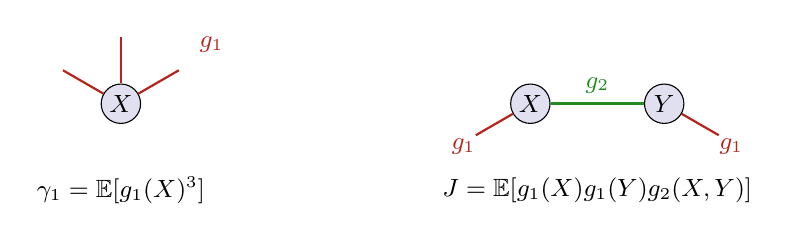
\begin{tikzpicture}[every node/.style={font=\small}]
\tikzset{v/.style={circle, draw, fill=NavyBlue!12, minimum size=5mm, inner sep=0}}
% gamma1 diagram: one vertex, three g1 legs
\begin{scope}
  \node[v] (a) at (0,0) {$X$};
  \foreach \ang in {150,90,30}
     \draw[BrickRed,thick] (a) -- ++(\ang:0.85);
  \node[BrickRed] at (1.15,0.75) {$g_1$};
  \node at (0,-1.1) {$\gamma_1=\E[g_1(X)^3]$};
\end{scope}
% J diagram: two vertices joined by g2, each with a g1 leg
\begin{scope}[xshift=5.2cm]
  \node[v] (x) at (0,0) {$X$};
  \node[v] (y) at (1.7,0) {$Y$};
  \draw[ForestGreen,very thick] (x) -- (y) node[midway,above]{$g_2$};
  \draw[BrickRed,thick] (x) -- ++(210:0.8); \node[BrickRed] at (-0.85,-0.55){$g_1$};
  \draw[BrickRed,thick] (y) -- ++(330:0.8); \node[BrickRed] at (2.55,-0.55){$g_1$};
  \node at (0.85,-1.1) {$J=\E[g_1(X)g_1(Y)g_2(X,Y)]$};
\end{scope}
\end{tikzpicture}
\caption{The two connected diagrams in the leading skewness \eqref{eq:c3}. Each
is an \Einsum{} contracting the Hoeffding components $g_1,g_2$ against the law
$p$. Higher cumulants and higher-order kernels give larger, non-chain diagrams
whose treewidth sets the cost.}
\label{fig:diagrams}
\end{figure}

\F{A concrete check} Take the $5$-letter kernel and law in
\texttt{code/exp7\_edgeworth.py}. The \Einsum{}s give
$\gamma_1=-0.0140$, $J=+0.0196$, $\zeta_1=0.128$, hence
\[
   c_3=\frac{\gamma_1+3J}{\zeta_1^{3/2}}=0.977,
   \qquad\text{whereas the single diagram}\quad
   \frac{\gamma_1}{\zeta_1^{3/2}}=-0.305
\]
has the \emph{wrong sign}. Computing the \emph{exact} cumulants of $U_n$ (via the
multinomial factorial moments, no asymptotics) confirms
$\lambda_3\sqrt n\to0.977$ as $n$ grows ($0.54,0.72,0.84,0.91,0.94$ at
$n=16,32,64,128,256$), and a $1.6\times10^{7}$-draw Monte-Carlo gives skewness
$0.092$ against the exact $\lambda_3=0.105$ at $n=64$. The two-diagram \Einsum{}
formula \eqref{eq:c3} is correct; the one-diagram shortcut is not.

% ===========================================================================
\section{The rate of the expansion}
% ===========================================================================

Because $\lambda_r=O(n^{-(r-2)/2})$, the successive terms of \eqref{eq:edgeworth}
shrink by a factor $n^{-1/2}$ each: the normal approximation errs at
$O(n^{-1/2})$ (the skewness term), adding it gives $O(n^{-1})$, adding the
kurtosis term gives $O(n^{-3/2})$, and so on. Figure~\ref{fig:edgeworth}
demonstrates both halves: the Edgeworth density captures the skew the normal
misses, and each extra term lowers the sup-distance to the true law at the
predicted rate.

\begin{figure}[h]
\centering
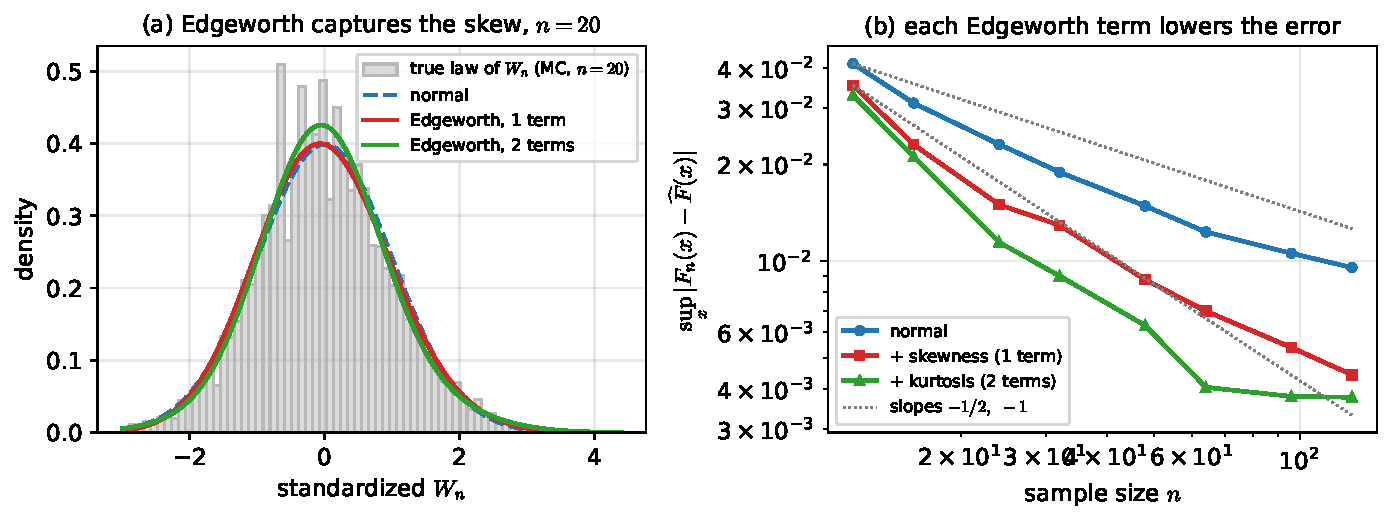
\includegraphics[width=\textwidth]{figures/edgeworth.pdf}
\caption{Edgeworth expansion of a $U$-statistic.
(a)~at $n=20$ the one- and two-term expansions track the (right-skewed) true law
that the normal cannot. (b)~the sup-error $\sup_x|F_n-\widehat F|$ against a
$1.6\times10^7$-draw Monte-Carlo truth: each Edgeworth term lowers it, along
slopes near $-\tfrac12$ and $-1$. (Discreteness of a small-alphabet statistic
caps the gain at small $n$; the coefficients themselves are exact.)}
\label{fig:edgeworth}
\end{figure}

\begin{principle}[what is being computed, and why it is the same calculus]
\label{obs:same}
The Edgeworth coefficients are cumulants; cumulants are connected sums of
diagrams; each diagram is an \Einsum{} of the kernel's Hoeffding components; and
the moment$\to$cumulant passage is the partition-lattice M\"obius inversion that
the companion paper already uses for $U\!\to\!V$. The treewidth of a diagram is
the cost of its contraction. So computing high-order distributional corrections
for high-order $U$-statistics \emph{is} the paper's treewidth-bounded \Einsum{}
problem, now indexed by cumulant order.
\end{principle}

% ===========================================================================
\section{Where treewidth bites, and what is next}
% ===========================================================================

\F{Higher order is where it is non-trivial} For an order-$2$ kernel the leading
diagrams are a point and an edge. For an order-$m$ kernel, the $r$-th cumulant is
a sum over connected diagrams on $r$ kernel-copies sharing arguments; these are
general graphs, the optimal contraction is the NP-hard treewidth problem, and the
heuristics of \texttt{opt\_einsum}/\texttt{cotengra} are exactly the tool for
enumerating them.\footnote{D.~G.~A.~Smith and J.~Gray (2018); J.~Gray and
S.~Kourtis (2021). The diagram/graph formalism for cumulants: P.~Major,
\emph{Multiple Wiener--It\^o Integrals}; S.~Janson, \emph{Gaussian Hilbert
Spaces}.} This is the genuine, non-chain home of the calculus -- unlike the
transfer-matrix series, nothing here collapses to a single quadratic form.

\F{Relatives in the same family} The same coefficients drive the
\emph{Cornish--Fisher} inversion (quantiles), the \emph{saddlepoint}
approximation (an exponential reordering of the same cumulants), and the
second-order correctness of the \emph{bootstrap}. The \emph{degenerate} case
($\zeta_1=0$, e.g.\ $\E[h(x,X)]\equiv\theta$) is a different regime entirely:
$n U_n$ converges to a weighted $\chi^2$ via the spectrum of the operator
$g_2$ -- an eigenvalue series rather than a normal one, and a natural next target.

\F{Honest caveats} The series is asymptotic, not convergent; the diagram count
grows fast with order; for lattice statistics a separate oscillatory correction
is needed (visible as the small-$n$ floor in Figure~\ref{fig:edgeworth}b); and
treewidth fixes the \emph{cost} of a coefficient, not its value.

\bigskip
\noindent\textit{Reproduce:} \texttt{python3 code/exp7\_edgeworth.py} computes the
diagram \Einsum{}s, the exact cumulants, and the figure; it prints the
verification of \eqref{eq:c3}.

\end{document}
